\documentclass[UTF8]{ctexart}
\usepackage{amsmath,amssymb,geometry,enumitem,mathtools,listings,graphicx,verbatim,framed,amsthm,subfigure}
\usepackage[usenames,dvipsnames]{color}
\usepackage{float}
\geometry{a4paper,scale = 0.7}	
\usepackage{xcolor}  	%高亮使用的颜色
\definecolor{commentcolor}{RGB}{85,139,78}
\definecolor{stringcolor}{RGB}{206,145,108}
\definecolor{keywordcolor}{RGB}{34,34,250}
%\definecolor{backcolor}{RGB}{220,220,220}
\newtheorem{theorem}{Theorem}
\newtheorem{lemma}{Lemma}
\newtheorem{corollary}{Corollary}
\newtheorem{definition}{Definition}
\usepackage{accsupp}
\newcommand{\emptyaccsupp}[1]{\BeginAccSupp{ActualText={}}#1\EndAccSupp{}}

\lstset{						%高亮代码设置
	language=C++,
	linewidth=0.9\linewidth,	  		%列表list宽度
	basicstyle=\ttfamily,				%tt无法显示空格
	commentstyle=\color{commentcolor},	%注释颜色
	keywordstyle=[1]\color{Blue}\bfseries,
	keywordstyle=[2]\color{Purple},
	keywordstyle=[3]\color{Blue}\underbar,
	stringstyle=\color{Purple},	%字符串颜色
	%showspaces=true,					%显示空格
	numbers=left,						%行数显示在左侧
	numberstyle=\normalsize\emptyaccsupp,		%行数数字格式
	numbersep=5pt,						%数字间隔
	frame=single,						%加框
	framerule=0pt,						%不划线
	escapeinside=@@,					%逃逸标志
	emptylines=1,						%
	xleftmargin=0.5em,					%list左边距
	%backgroundcolor=\color{backcolor},	%列表背景色
	tabsize=4,							%制表符长度为4个字符
	%gobble=4,							%忽略每行代码前4个字符
	upquote,
}


\title{Manderbrot Set 的生成和探索}
\author{毕嘉文 \\ 数学与应用数学\ 3190105194}
\date{\today}
\begin{document}
\maketitle
\begin{abstract}
在本文中,我们简单介绍Mandelbrot Set的历史发展和相关数学知识,使用C++复现了Mandelbrot Set的生成算法,并且尝试扩展生成色彩更丰富的图片。
\end{abstract}
\section{背景介绍}

Mandelbrot 集起源于20 世纪初,法国数学家 Pierre Fatou 和 Gaston Julia 首次研究的复动力学领域。 
1978 年,罗伯特·W·布鲁克斯 (Robert W. Brooks) 和彼得·马特尔斯基 (Peter Matelski) 首次定义并绘制了这种分形,作为克莱因群研究的一部分。 
\cite{4th1981riemann} 
1980 年 3 月 1 日,Benoit Mandelbrot 在位于纽约约克镇高地的 IBM Thomas J. Watson 研究中心首次见到了该集合的可视化。 \cite{Taylor2008}
Mandelbrot 在 1980 年发表的一篇文章中研究了二次多项式的参数空间。 \cite{https://doi.org/10.1111/j.1749-6632.1980.tb29690.x}
Mandelbrot 集的数学研究真正开始于数学家 Adrien Douady 和 John H. Hubbard \cite{Douady1984tudeDD} 的工作,
他们建立了它的许多基本性质,并为 Mandelbrot 命名该集以纪念他在分形几何方面的有影响力的工作.

1986年左右,数学家 Heinz-Otto Peitgen 和 Peter Richter 通过照片、书籍\cite{peitgen1986beauty} 以及德国歌德学院的国际巡回展览来宣传该系列。

1985 年 8 月,由不来梅大学的 Peitgen、Richter 和 Saupe 创作的Scientific American的封面文章\cite{10.2307/24967754} 向广大读者介绍了计算 Mandelbrot 集的算法。在 1980 年代中期,计算机变得足够强大,可以以高分辨率绘制和显示Mandelbrot 集,此时它在计算机图形方面的美学价值得以展现。

Douady 和 Hubbard 的工作正巧遇到了科学从业者们对复杂动力学和抽象数学的兴趣大幅增加,
从那时起,对 Mandelbrot 集的研究就是该领域的核心了。
\section{数学理论}

\subsection{定义}
Mandelbrot 集可用复二次多项式来定义:\begin{align}
f_c(z) = z^2 + c
\end{align}
其中$c$是一个复数参数。从$z = 0$开始对$f_c(x)$进行迭代:\begin{align}
z_{n+1} = z_n^2 + c
\end{align}
迭代后得到如下序列$$
(0,\ f_c(0),\ f_c(f_c(0)). \ \cdots )
$$
不同的参数$c$可以使序列的绝对值逐渐发散到无穷大,也可能收敛到有限的区域内。Mandelbrot 集就是使得序列不延伸到无限大的所有复数$c$ 的集合。

\subsection{基本性质}
Mandelbrot 集是一个紧集,因为它是闭合的并且包含在以原点为中心的半径为 2 的闭合圆盘中。 
更具体来说,点 $c$ 属于 Mandelbrot 集当且仅当 $\vert z_{n}\vert\leq 2,\  \forall n\geq 0$。 
由于 $c = z_1$,因此 $\vert c\vert\leq 2$,即$c$将始终位于原点周围半径为 $2$ 的封闭圆盘中。


$M$ 与实轴的交点正好是区间 $[-2,\dfrac1{ 4}]$, 沿着这个区间的参数可以与真实逻辑族的参数一一对应,i.e.\begin{align}
x_{n+1} = rx_n(1-x_n), \ r\in[1,4] \end{align}
相应有\begin{align}
z = r(\dfrac12 - x), c = \dfrac{r}2 (1-\dfrac{r}2)
\end{align}


我们通常猜测 Mandelbrot 集是局部连通的。 这个著名的猜想被称为 MLC(Mandelbrot locally connected)猜想。


Mandelbrot 集在 Misiurewicz 点附近放大后是自相似的。 
在收敛到极限集的意义上,它也被认为关于广义Feigenbaum点(例如 $-1.401155$ 或 $-0.1528 + 1.0397i$)是自相似的。 [21] [22] 
Mandelbrot 集通常不是严格自相似的,但它是准自相似的,因为可以在任意小尺度上找到其自身略有不同的相似形,但Mandelbrot 的这些相似形都略有不同。
\section{代码及算法}
以下为Mandelbrot Set的基本生成算法:
\begin{lstlisting}
for(int i = 0; i < height; i++){
	for(int j = 0; j < width; j++){
		complex c = some formula of i and j;
		complex z = 0;
		for(int n = 0; n < N; n++){
			if(squared_modulus(z) > 4){
				image[i][j] = black;
				goto label;
			}
			z = z * z + c;
		}
		image[i][j] = white;
		label:{}
	}
}
\end{lstlisting}
在此基础上,我们可以尝试对不同迭代次数的点染上不同的颜色,详情请见代码。
\section{数值算例}
考虑到pdf文件大小,在这里我仅展示两张低像素的图片,若想查看更大像素的图片可以前往image文件夹。
\begin{figure}[H]
	\centering
	\begin{minipage}{0.48\textwidth}
		\centering
		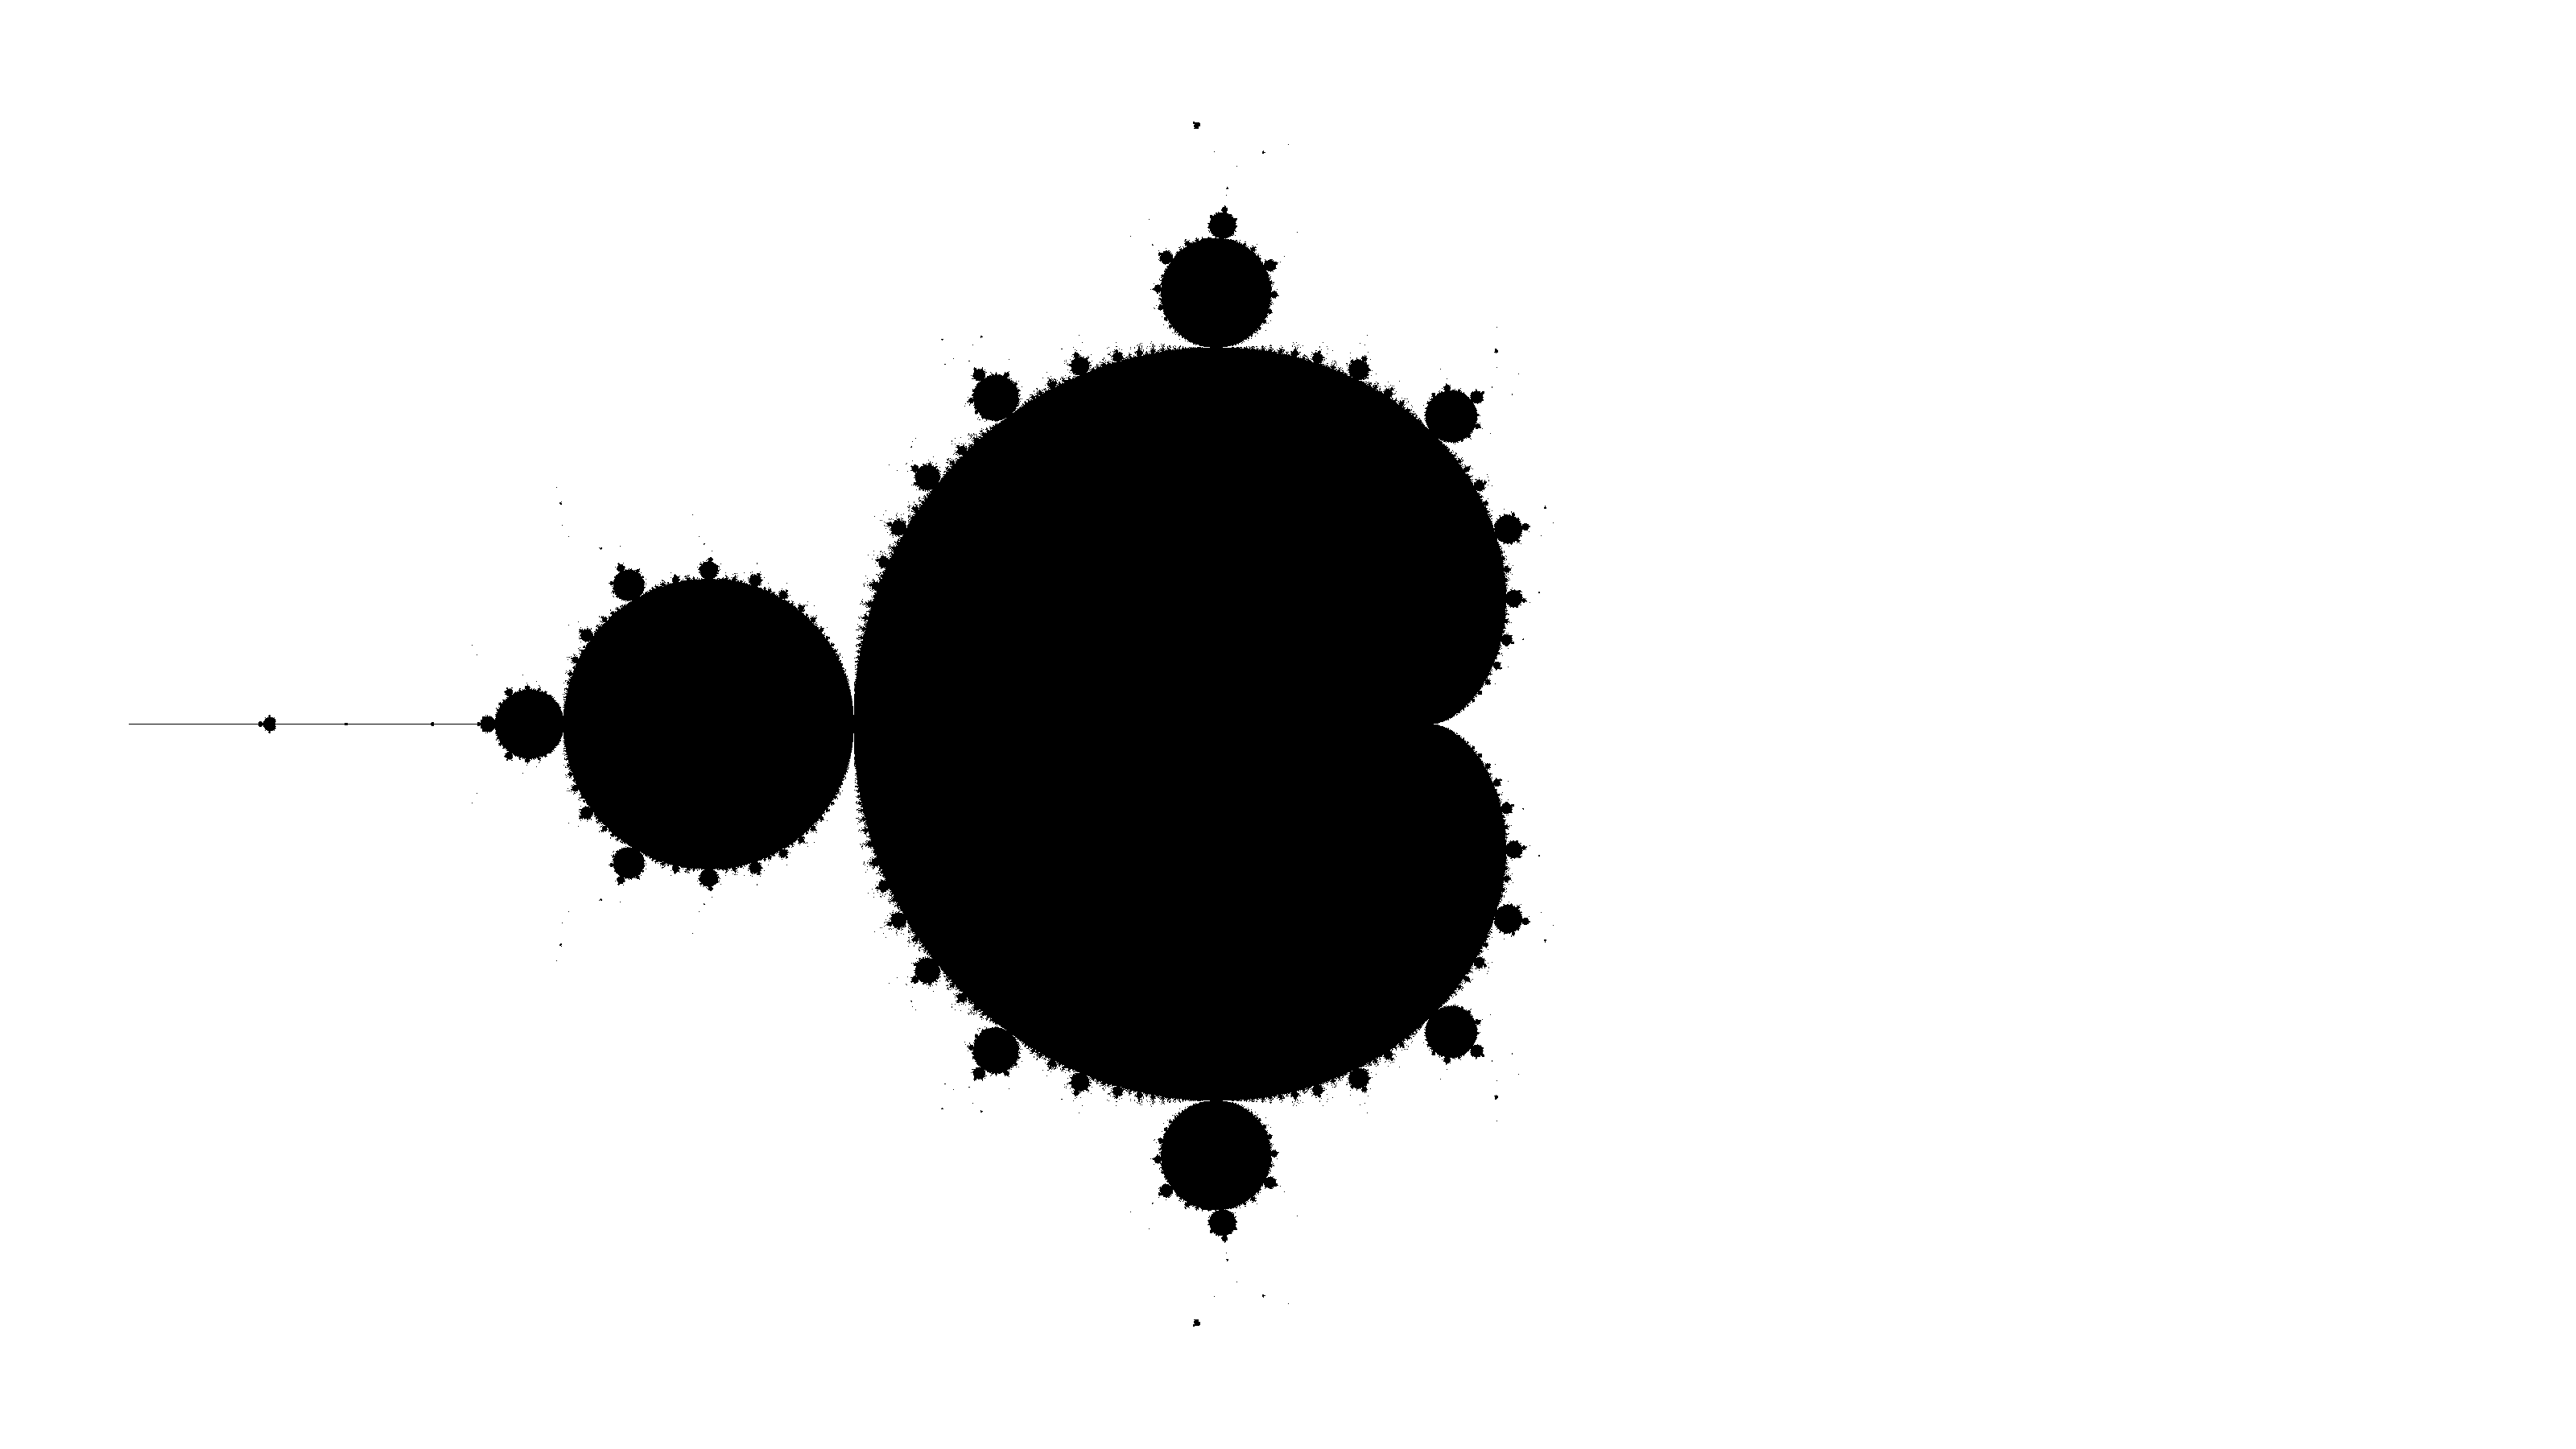
\includegraphics[width=1\linewidth]{../image/tmp_origin.png}
		\caption{初始染色}
	\end{minipage}
	\begin{minipage}{0.48\textwidth}
		\centering
		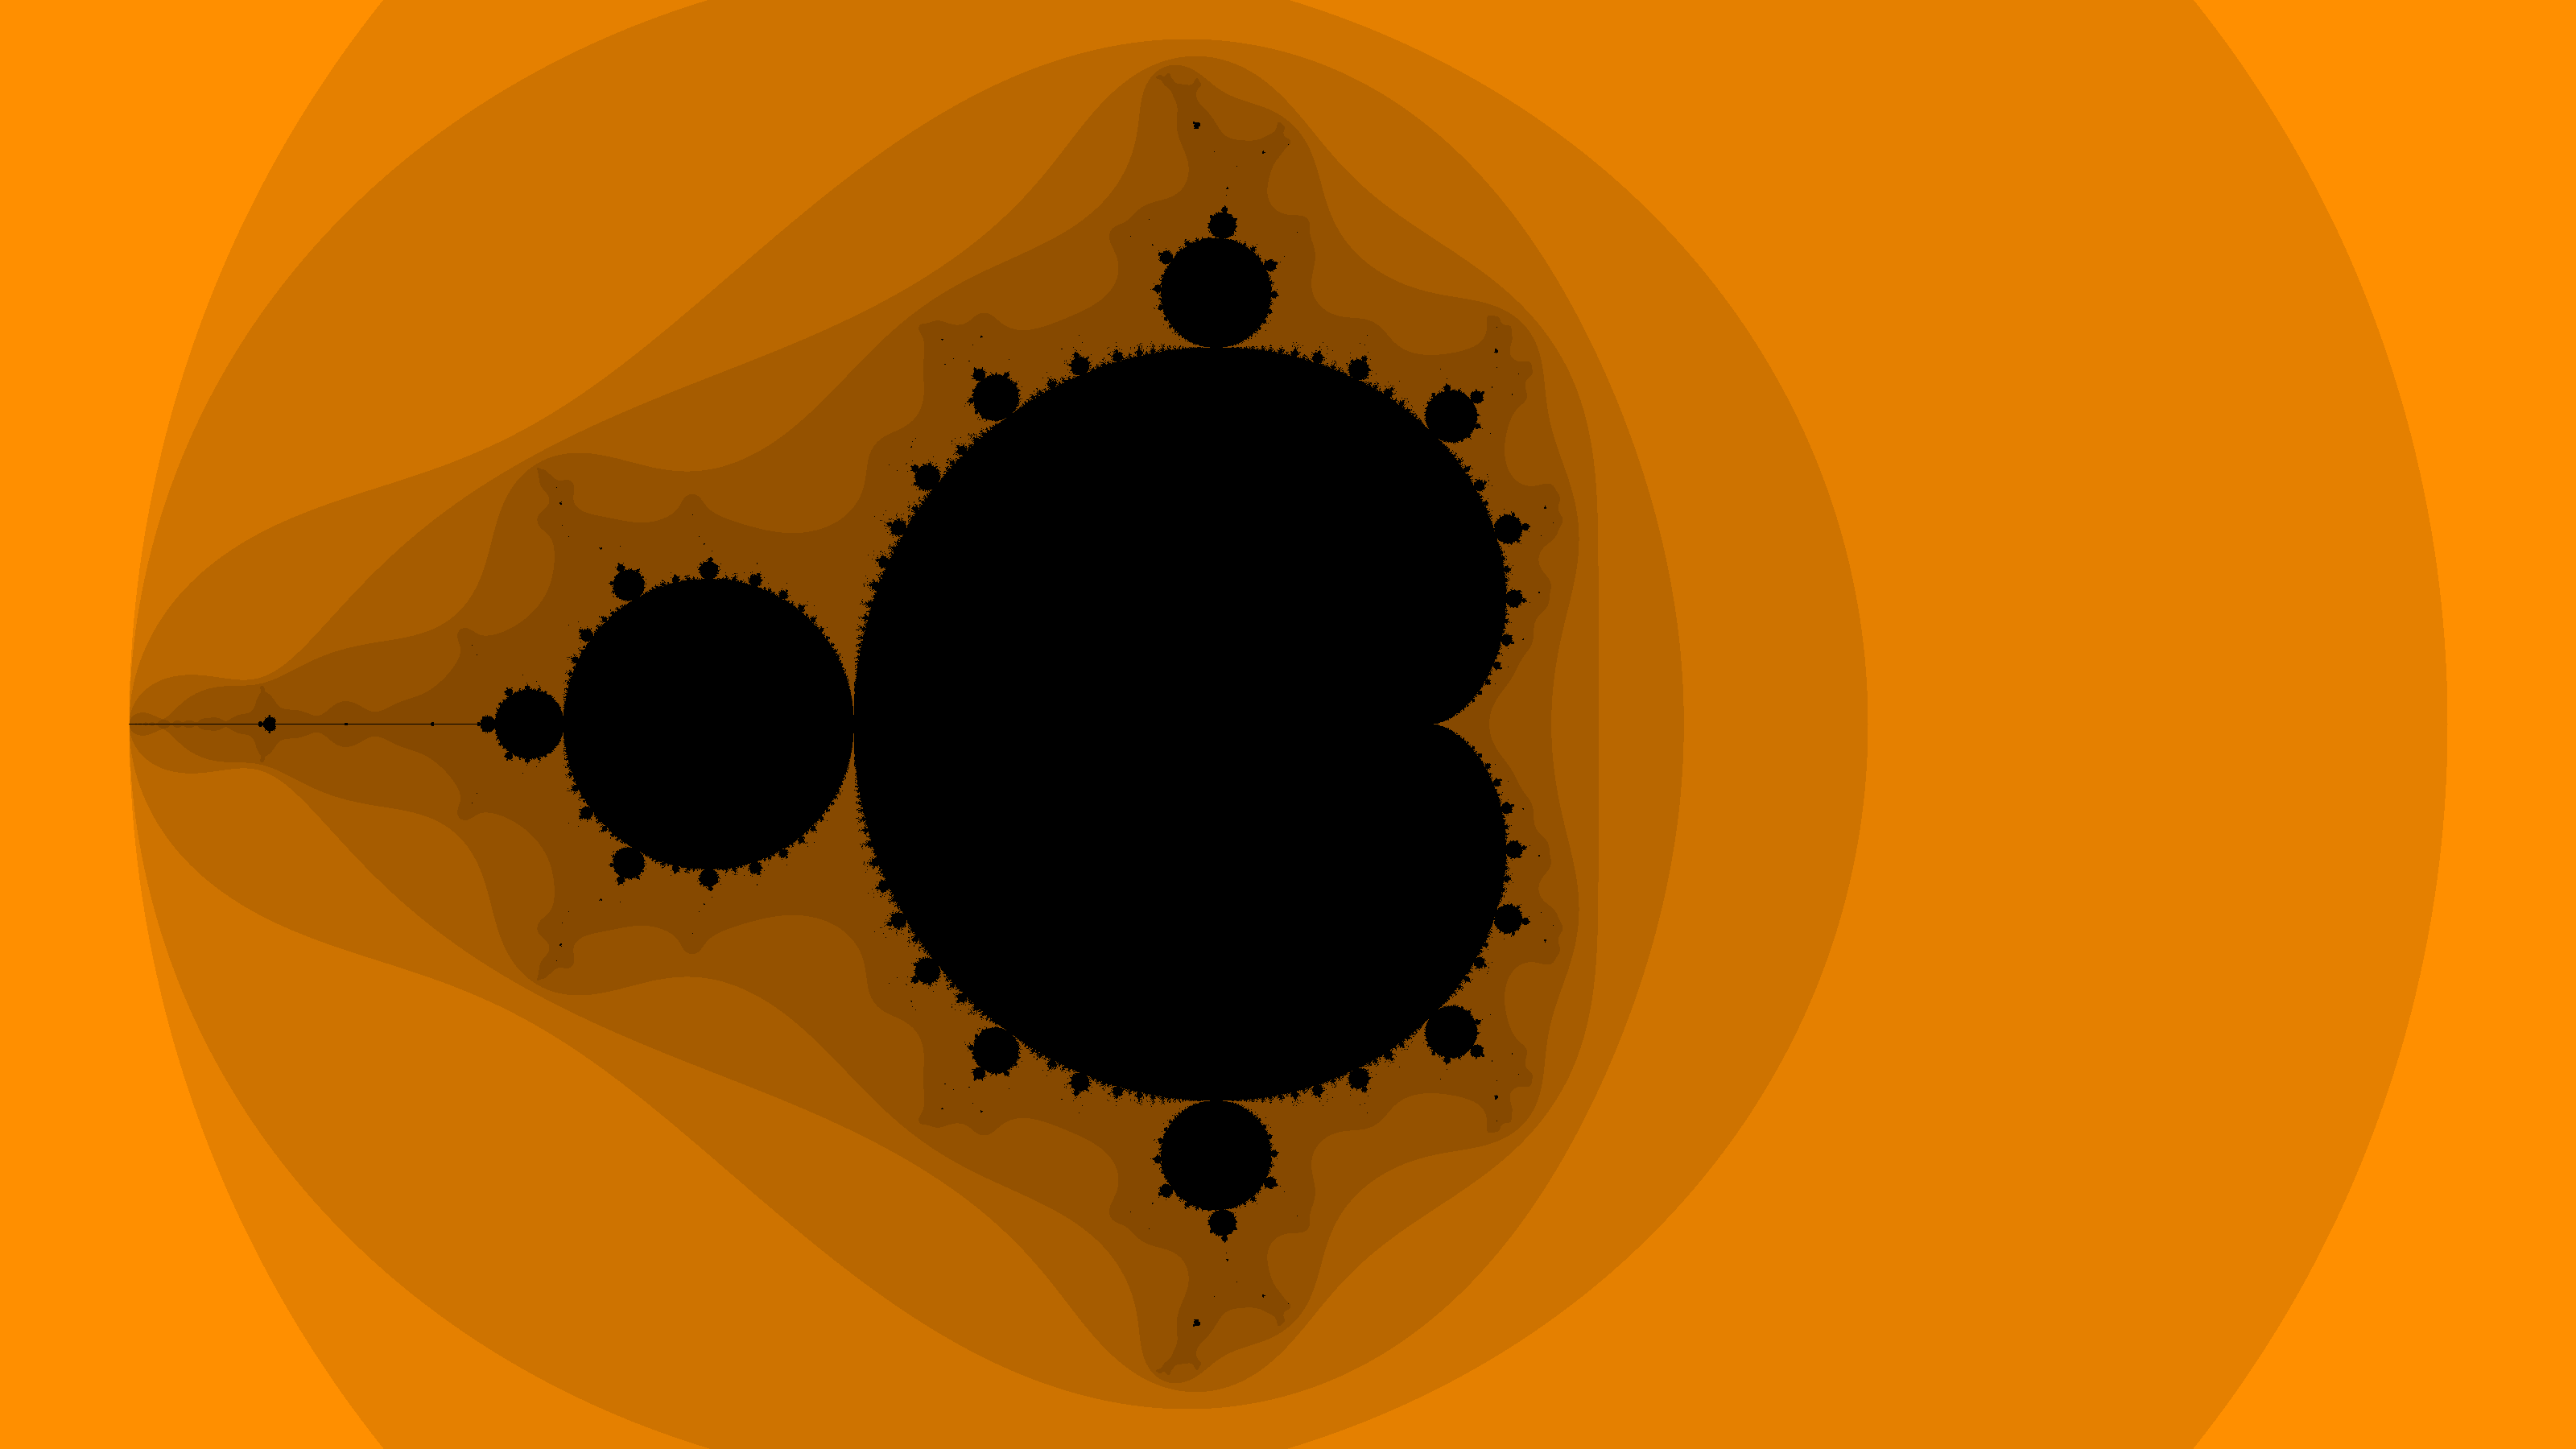
\includegraphics[width=1\linewidth]{../image/tmp_colored.png}
		\caption{使用颜色008fff}
	\end{minipage}
\end{figure}
\section{结论}
根据运行结果,我们可以验证上述提到的一些基本性质,比如自相似性,局部连通性等。
\bibliographystyle{plain}
\bibliography{work}
\end{document}
